\section{Directed Search Algorithmus}
Der directed Search Algorithmus unterst�tzt DART bei der Findung von Eingabevektoren. �hnlich wie bei der dynamischen
Generierung von Testdaten wird das Programm zun�chst mit zuf�lligen Werten gestartet \cite{godefroid2005dart, korel1990dynamic}.
F�r jede Ausf�hrung wird nun ein neuer Inputvektor gebildert. Wie bereits erl�utert, ist der Inputvektor entscheidend
f�r die Reihenfolge der Statements die ausgef�hrt werden. Dieser Inputvektor kann dann f�r die n�chsten Iterationen genutzt werden. Zeitgleich werden alle Pfadbeschr�nkungen notiert,
welche f�r den zuf�lligen Inputvektor nicht positiv als Ergebnis haben \cite{godefroid2005dart}. Aus dem vorher genannten
Beispiel aus Listing \ref{lst:function-fh}

Anschlie�end wird f�r die n�chste Ausf�hrung
ein neuer Input Vektor berechnet. Dieser Input Vektor basiert dabei auf Werten aus den vorherigen Berechnungen, um die
Zweigbedingungen zu l�sen \cite{godefroid2005dart}.
Dies geschieht, damit das Programm zu einer entsprechenden Node gelenkt werden kann, was �hnlich zum Suchalgorithmus
von Korel ist \cite{korel1990dynamic}. Dieser Vorgang wird nun so oft wiederholt, bis alle m�glichen Pfade ausgef�hrt
wurden \cite{godefroid2005dart}.

Hierbei wird nicht nur die konkrete Ausf�hrung des Programms selbst durchgef�hrt, sondern auch die Ausf�hrung des Programms
mit \textit{symbolischen Werten}. King sagt, dass es sich bei der Ausf�hrung mithilfe von symbolischen Werten um eine
Erweiterung der normalen Ausf�hrung handelt \cite{king1976symbolic}. Somit werden f�r eine Sprache die Operatoren derart
erweitert, dass sie ebenso symbolische Werte annehmen und verarbeiten k�nnen. Diese produzieren dann \textit{symbolic formulas}
als Ausgabe \cite{king1976symbolic}, welche wiederum von DART genutzt werden k�nnen, sodass daraus \textit{Constraints}
abgeleitet werden k�nnen \cite{godefroid2005dart}.


Der DART Algorithmus arbeitet also folgenderma�en. Wie man in \ref{fig:testdriver-dart} erkennen kann, werden zun�chst
ein Stack und der Inputvektor zur�ckgesetzt, sodass dieser durch den Directed Search Algorithmus berechnet werden kann

\begin{figure}[h!]
    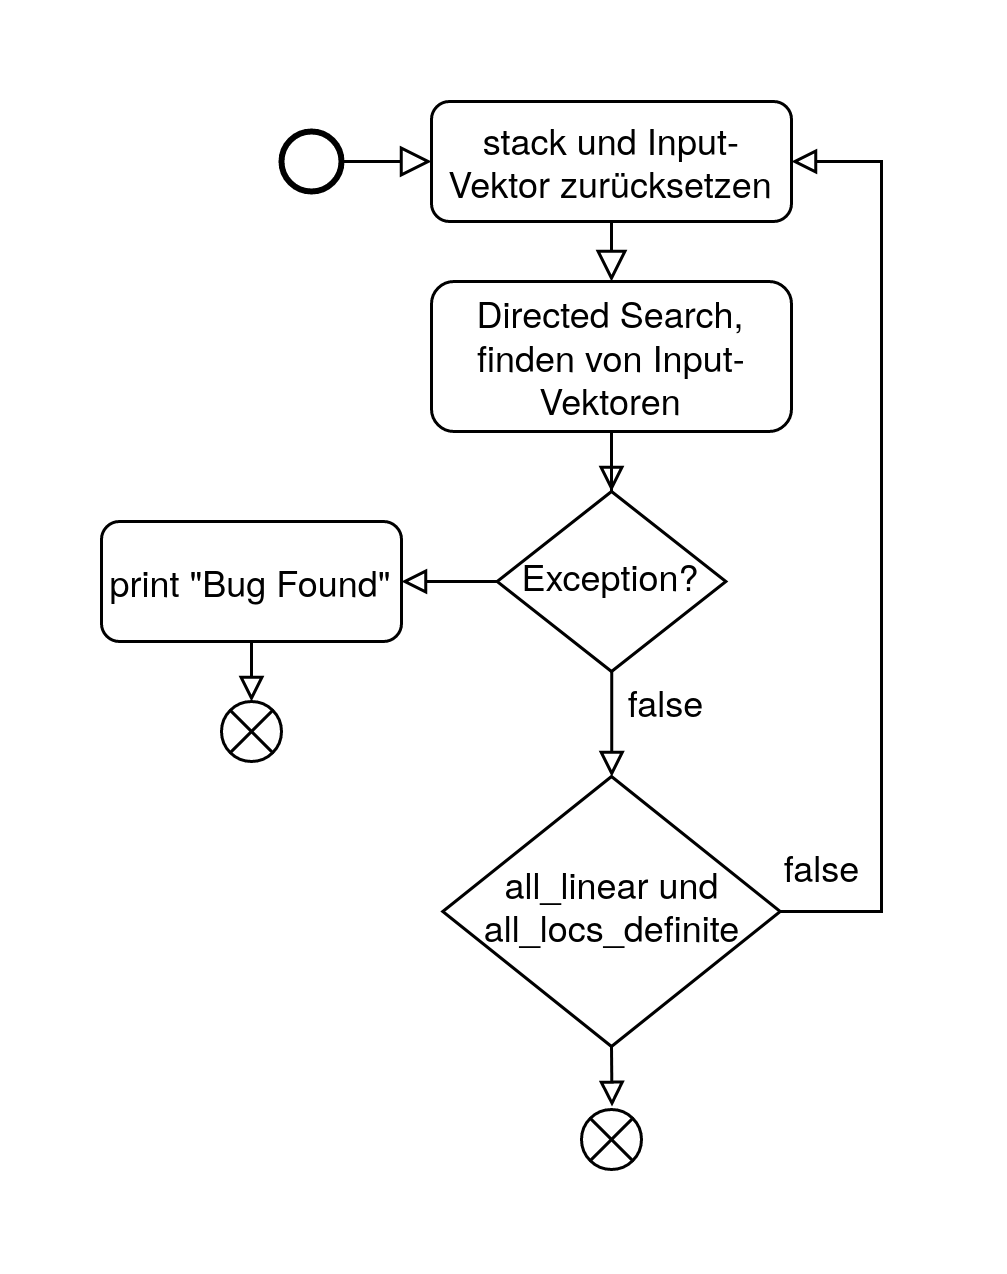
\includegraphics[scale=0.2]{Bilder/dart/testdriver.png}
    \caption{Test Driver nach Godefroid}
    \label{fig:testdriver-dart}
\end{figure}
